\chapter{体系结构初步}\thispagestyle{empty}
    \begin{summary}
        \begin{compactitem}
            \item 了解体系结构的简要发展史,熟悉 RISC、CISC 的区别和应用。了解基本的门电路、算术运算器、选择器、触发器和寄存器的原理和实现。
            \item 熟悉 Y86-64 “体系结构”中,各种指令的编码规则(包括操作数、指令子类型等),会将汇编代码和指令编码相互转换。简单了解 MIPS 体系结构。
            \item 在上一项的基础上,理解并熟练\uwave{记忆} Y86-64 SEQ 处理器执行各种指令的几个阶段及其详细的功能(含重要的中间状态变化)。理解并熟练\uwave{记忆} Y86-64 顺序处理器的实现(HCL)。
            \item 知道流水线设计的通用原理,会进行相关的计算和分析。
            \item 在 SEQ 处理器的基础上,理解并熟练\uwave{记忆} Y86-64 PIPE 处理器和 SEQ 处理器的不同。会分析流水线冒险和转发逻辑。理解并熟练\uwave{记忆} Y86-64 顺序处理器的实现(HCL)。
            \item 理解编译器进行程序性能优化的常见变换手段和不进行优化的保守原因。会通过数据相关图和关键路径分析对性能进行计算(如 CPE 数值)。
        \end{compactitem}
    \end{summary}

    \begin{problems}
        \pro 下列描述更符合(早期)RISC 还是 CISC?
            \qn 指令机器码长度固定。
            \qn 指令类型多、功能丰富。
            \qn 不采用条件码。
            \qn 实现同一功能,需要的汇编代码较多。
            \qn 译码电路复杂。
            \qn 访存模式多样。
            \qn 参数、返回地址都使用寄存器进行保存。
            \qn x86-64。
            \qn MIPS。
            \qn 广泛用于嵌入式系统。
            \qn 已知某个体系结构使用 \verb|add R1, R2, R3| 来完成加法运算。当要将数据从寄存器 \verb|S| 移动至寄存器 \verb|D| 时,需要使用 \verb|add S, #ZR, D| 进行操作(\verb|#ZR| 是一个恒为 0 的寄存器)。
            \qn 已知某个体系结构提供了 \verb|xlat| 指令,它以一个固定的寄存器 \verb|A| 为基地址,以另一个固定的寄存器 \verb|B| 为偏移量,在 \verb|A| 对应的数组中取出下标为 \verb|B| 的项的内容,放回寄存器 \verb|A| 中。
        \sol 依次为 RISC、CISC、RISC、RISC、CISC、CISC、RISC、CISC、RISC、RISC、RISC、CISC。这里对于 1,固定长的指令译码电路简单;通常 CISC 有变长指令,例如 x86 中清零用 \verb|xor|,因为这样可以节省指令长度。对于 10,嵌入式系统是指可穿戴设备、物联网之类的小设备,功能简单且需要省电,因此处理器电路不用太复杂。
        \pro 写出下列电路对应的逻辑表达式:
        \begin{figure}[H]
            \centering
            \begin{tikzpicture}[
                GateCfg/.style={
                    logic gate inputs={normal, normal, normal},
                    draw
                }
            ]
                \path (0,0) node[and gate US, GateCfg] (AND1) {} ++(2,-2) node[and gate US, GateCfg] (AND2) {} ++(5,1) node[or gate US, GateCfg] (OR1) {} (AND1.input 3) ++(-1,0) node[not gate US, draw] (N1) {} (AND2.input 3) ++(-1,0) node[not gate US, draw] (N2) {} (AND2.input 1 -| N1) node[not gate US, draw] (N3) {};
        
                \draw (OR1.input 1) -- ++(-1.5,0) |- (AND1.output) (OR1.input 3) -- ++(-1.5,0) |- (AND2.output) (N2.output) -- (AND2.input 3) (N1.output) -- (AND1.input 3) (N3.output) -- (AND2.input 1) (AND1.input 1) -- ++(-3,0) coordinate (init) node[anchor=east] {\texttt{A}} node[pos=0.6] (temp) {} (N1-| temp) ++(0,5pt) edge (temp.center) arc (90:-90:5pt) |- (N3.input) (init |- N1) node[anchor=east] {\texttt{B}} -- (N1.input) node[pos=0.4] (temp2) {} (temp2.center) |- (N2.input) (OR1.output) -- ++(2,0) node [midway,anchor=south]{\texttt{f(A, B)}};
            \end{tikzpicture}
        \end{figure}
        \sol \verb+f(A, B) = (!A && B) || (A && !B)+。
        \pro 根据 Y86-64 体系结构完成下表中的更新逻辑:
        \begin{table}[H]
            \tt
            \centering
            \begin{tabular}{|c|c|c|c|}
                \hline
                &  & call & jXX \\ \hline
                \multirow{4}{*}{Fetch (F)} & icode, ifun & {\qquad \qquad \qquad \qquad} & {\qquad \qquad \qquad \qquad} \\ \cline{2-4} 
                & rA, rB &  &  \\ \cline{2-4} 
                & valC &  &  \\ \cline{2-4} 
                & valP &  &  \\ \hline
                \multirow{2}{*}{Decode (D)} & valA, srcA &  &  \\ \cline{2-4} 
                & valB, srcB &  &  \\ \hline
                \multirow{2}{*}{Execute (E)} & valE &  &  \\ \cline{2-4} 
                & Cond Code &  &  \\ \hline
                Memory (M) & valM &  &  \\ \hline
                \multirow{2}{*}{Writeback (W)} & dstE &  &  \\ \cline{2-4} 
                & dstM &  &  \\ \hline
                PC & PC &  &  \\ \hline
            \end{tabular}
        \end{table}
        \sol 首先确定 \verb|call V| 和 \verb|jXX V| 两个指令都长 9 字节,然后按运算逻辑进行填写即可。没有填写的空格表示不需要填。
        \begin{table}[H]
            \tt
            \centering
            \begin{tabular}{|c|c|c|c|}
                \hline
                &  & call & jXX \\ \hline
                \multirow{4}{*}{Fetch} & icode:ifun & icode:ifun <- M1[PC] & icode:ifun <- M1[PC] \\ \cline{2-4} 
                & rA, rB &  &  \\ \cline{2-4} 
                & valC & valC <- M8[PC+1] & valC <- M8[PC+1] \\ \cline{2-4} 
                & valP & valP <- PC+9 & valP <- PC+9 \\ \hline
                \multirow{2}{*}{Decode} & valA &  &  \\ \cline{2-4} 
                & valB & valB <- R[\%rsp] &  \\ \hline
                \multirow{2}{*}{Execute} & valE & valE <- valB+(-8) &  \\ \cline{2-4} 
                & Cond Code &  & Cnd <- Cond(CC, ifun) \\ \hline
                Memory (M) & valM & M8[valE] <- valP &  \\ \hline
                \multirow{2}{*}{Writeback} & dstE & R[\%rsp] <- valE &  \\ \cline{2-4} 
                & dstM &  &  \\ \hline
                PC & PC & PC <- valC & PC <- Cnd?valC:valP \\ \hline
            \end{tabular}
        \end{table}
        \pro 已知 \verb|valC| 为指令中的常数值,\verb|valM| 为访存得到的数据,\verb|valP| 为 \verb|PC| 自增得到的值,完成以下的 PC 更新逻辑:
        \begin{minted}[frame=single, fontsize=\small]{text}
    int new_pc = [
        icode == ICALL : _____;
        icode == IJXX && Cnd: _____;
        icode == IRET : _____;
        1: _____;
    ];
        \end{minted}
        \sol 此题顺着上一题的填写就很容易写出了。
        \begin{minted}[frame=single, fontsize=\small]{text}
    int new_pc = [
        icode == ICALL : valC;
        icode == IJXX && Cnd: valC;
        icode == IRET : valM;
        1: valP;
    ];
        \end{minted}
        \pro 判断下列说法的正确性:
            \qn 流水线的深度越深,总吞吐率越大,因此流水线应当越深越好。
            \qn 流水线的吞吐率取决于最慢的流水级,因此流水线的划分应当尽量均匀。\qn 假设寄存器延迟为 \SI{20}{ps},那么总吞吐率不可能达到或超过 \SI{50}{GIPS}。
            \qn 数据冒险总是可以只通过转发来解决。
            \qn 数据冒险总是可以只通过暂停流水线来解决。
        \sol 分别是错误(深度会影响冒险问题和电路复杂性,以及吞吐量有上界)、正确、正确、错误(load-use 冒险)、正确。
        \pro 一条三级流水线,包括延迟为 \SI{50}{ps}、\SI{100}{ps}、\SI{100}{ps} 的三个流水级,每个寄存器的延迟为 \SI{10}{ps}。那么这条流水线的总延迟是 \rule{2.5cm}{0.25mm} ps,吞吐率是 \rule{2.5cm}{0.25mm} GIPS。
        \sol 总延迟为 $100+100+100+3 \times 10 = \SI{330}{ps}$,吞吐率为 $1/330 = \SI{9.09}{GIPS}$。
        \pro 在下图中,A\textasciitilde H 为 8 个基本逻辑单元,图中标出了每个单元的延迟,以及用箭头标出了单元之间的数据依赖关系。寄存器的延迟均为 \SI{10}{ps}。
        \begin{figure}[H]
            \centering
            \begin{tikzpicture}
                \draw[draw=black] (0,0) rectangle ++(1,1.5);
                \node[align=center] at (0.5,0.75) {A \\ \SI{40}{ps}};
                \draw[draw=black] (2,0) rectangle ++(1,1.5);
                \node[align=center] at (2.5,0.75) {B \\ \SI{30}{ps}};
                \draw[draw=black] (4,0) rectangle ++(1,1.5);
                \node[align=center] at (4.5,0.75) {C \\ \SI{40}{ps}};
                \draw[draw=black] (6,0) rectangle ++(1,1.5);
                \node[align=center] at (6.5,0.75) {D \\ \SI{20}{ps}};
                \draw[-{Stealth[angle'=45]}] (1,0.75) -- (2,0.75);
                \draw[-{Stealth[angle'=45]}] (3,0.75) -- (4,0.75);
                \draw[-{Stealth[angle'=45]}] (5,0.75) -- (6,0.75);
                \draw[-{Stealth[angle'=45]}] (7,0.75) -- (8,0.75);

                \begin{scope}[shift={(0,-2.5)}]
                    \draw[draw=black] (0,0) rectangle ++(1,1.5);
                    \node[align=center] at (0.5,0.75) {E \\ \SI{20}{ps}};
                    \draw[draw=black] (2,0) rectangle ++(1,1.5);
                    \node[align=center] at (2.5,0.75) {F \\ \SI{60}{ps}};
                    \draw[draw=black] (4,0) rectangle ++(1,1.5);
                    \node[align=center] at (4.5,0.75) {G \\ \SI{40}{ps}};
                    \draw[draw=black] (6,0) rectangle ++(1,1.5);
                    \node[align=center] at (6.5,0.75) {H \\ \SI{30}{ps}};
                    \draw[-{Stealth[angle'=45]}] (1,0.75) -- (2,0.75);
                    \draw[-{Stealth[angle'=45]}] (3,0.75) -- (4,0.75);
                    \draw[-{Stealth[angle'=45]}] (5,0.75) -- (6,0.75);
                    \draw[-{Stealth[angle'=45]}] (7,0.75) -- (8,0.75);
                \end{scope}

                \draw[draw=black] (8,-2.5) rectangle ++(0.5,4);
                \node[align=center] at (8.25,-0.5) {R \\ E \\ G};
                \draw[-{Stealth[angle'=45]}] (1,0) -- (2,-1);
                \draw[-{Stealth[angle'=45]}] (5,-1) -- (6,0);
            \end{tikzpicture}
        \end{figure}
        \qn 计算目前的电路的总延迟。
        \qn 通过插入寄存器,可以对这个电路进行流水化改造。现在想将其改造为两级流水线, 为了达到尽可能高的吞吐率,问寄存器应插在何处?获得的吞吐率是多少?
        \qn 现在想将其改造为三级流水线,问最优改造所获得的吞吐率是多少?
        \sol 这里有多条数据通路,其总延迟由最高延迟的通路 $\mathrm A \to \mathrm F \to \mathrm G \to \mathrm H$ 决定,延迟是 $40+60+40+30+10 = \SI{180}{ps}$。插入寄存器使得其成为二级流水线,要求每一个通路都成为二级流水线,相当于多条单通路流水线求 $\max \min$。这里,通路 A\textasciitilde D 应当在 BC 之间插入寄存器;通路 E\textasciitilde H 应当在 FG 之间插入寄存器,此时各条数据通路都已经是二级的,最高单级延迟为 $40+60+10 = \SI{110}{ps}$,吞吐量 \SI{9.09}{GIPS}。对于三级流水线也是同样的道理,先考虑最慢通路 AFGH,它的两个寄存器应该放到 AF 和 FG 之间,此时 EFGH 的寄存器只能插在 EF 间(否则 AFGH 成为四级)。ABCD 通路的寄存器应插在 AB、BC 之间。综上,插入位置是 AB、AF、EF、BC、FG 之间,最高单级延迟 \SI{80}{ps},吞吐量 \SI{12.5}{GIPS}。
        \pro 一个只使用流水线暂停、没有数据前递的 Y86-64 流水线处理器,为了执行以下的语句,至少需要累计停顿多少个周期?
            \qn
            \begin{minted}[frame=single, fontsize=\small]{text}
    irmovq   $1, %rax
    irmovq   $2, %rbx
    addq     %rax, %rcx
    addq     %rbx, %rdx
    halt
            \end{minted}
            \qn
            \begin{minted}[frame=single, fontsize=\small]{text}
    rrmovq   %rax, %rdx
    mrmovl   (%rcx), %rax
    addq     %rdx, %rax
    halt
            \end{minted}
            \qn
            \begin{minted}[frame=single, fontsize=\small]{text}
    irmovq   $0x40, %rax
    mrmovq   (%rax), %rbx
    subq     %rbx, %rcx
    halt
            \end{minted}
        \sol (1)为 2 个。第 5 个时钟周期结束以后,第 3 行代码才能开始译码。而原来第 3 行在第 4 个时钟周期开始译码,因此需要 2 周期停顿。(2)为 3 个。1、3 两行,2、3 两行均有数据相关。为了解决 1、3 两行的数据相关,需要额外的 2 个停顿;为了解决 2、3 两行的数据相关,需要额外 3 个停顿,因此需要将第 3 行的指令停顿 3 个周期。(3)为 6 个。1、2 两行的数据相关,需要额外 3 个停顿才能解决;2、3 两行的数据相关,需要额外 3 个停顿才能解决,因此需要将 2、3 行的指令各停顿 3 个周期,共 6 个周期。
        \pro 考虑 Y86-64 中的 \verb|ret| 与 \verb|jXX| 指令。\verb|jXX| 总是预测分支跳转。
            \qn 写出流水线需要处理 \verb|ret| 的条件(\verb|ret| 对应的常量为 \verb|IRET|)。
            \qn 写出发现上述条件以后,各阶段的流水线寄存器应设置的状态。
            \qn 写出流水线需要处理 \verb|jXX| 分支错误的条件(\verb|jXX| 对应的常量为 \verb|IJXX|)。
            \qn 写出发现上述条件以后,各阶段的流水线寄存器应设置的状态。
            \qn 同时考虑上述两条指令,补全下面有关下一条指令地址 \verb|f_pc| 的控制逻辑。
            \begin{minted}[frame=single, fontsize=\small]{text}
    int f_pc = [
        M_icode == IJXX && !M_Cnd : __________;
        W_icode == IRET : __________;
        1 : __________;
    ];

    # 已知有如下的代码,其中 valC 为指令中的常数值
    # valM 为访存得到的数据,valP 为 PC 自增得到的值:
    int f_predPC = [
        f_icode in { IJXX, ICALL } : f_valC;
        1 : f_valP;
    ];
    int d_valA = [
        D_icode in { ICALL, IJXX } : D_valP; # Use incremented PC
        # ...省略部分数据前递代码
        1 : d_rvalA; # Use value read from register file
    ]; 
            \end{minted}
        \sol 此题帮助你理解并记忆 \verb|pipe.hcl| 的实现。
        
        第一问。\verb|ret| 指令在通过 D、E、M 三个阶段时,流水线都有问题(都在取错指令):其中 D 阶段开始取错指令,M 阶段行将结束时才能拿到返回地址,进行转发。所以应该填写 \verb|IRET in {D_icode, E_icode, M_icode}|。顺便一提,\verb|load-use| 的访存指令通过 E 时,前一阶
        段的 D 才出现问题,而访存通过 M 之后才能转发信号。\verb|mispredicted jXX| 影响最短,E 时可能发现预测错误,E 结束之后也就能确定下一条指令位置了。所以 \verb|load-use| 的检测条件是 \verb|E_icode in { IMRMOVQ, IPOPQ }|,等等。

        第二问为 \verb|ret| 的处理方法。它在 D 时,前面处于 F 阶段的指令已经出现了问题。那 F 阶段是 stall 还是bubble 呢?我们指出 F 阶段是不可以 bubble 的(Y86-64 实现中的 bubble 是将寄存器设为 reset 状态;F 仅仅是预测的 PC,无法模拟出 \verb|nop| 的状态)。这样我们令 F 阶段stall(反复地尝试取指),根据暂停规律\footnote{若某阶段是 stall,则下一阶段如无暂停必要就是 bubble,最后一个暂停后一定是 bubble;stall 的前一阶段一定是 stall。},后一阶段应该是 bubble,其余 normal。这样一来 \verb|ret| 到 E、M 两个阶段时,都是让 F stall,D bubble,实际上连续产生了三个气泡。等 M 结束后,下一次取指才能正常,冒险结束。所以答案为(注意对于 \verb|ret|,这个表实际上是三个一样的表)
        \begin{table}[H]
            \centering
            \begin{tabular}{|c|c|c|c|c|}
                \hline
                F & D & E & M & W \\ \hline
                stall & bubble & normal & normal & normal \\ \hline
            \end{tabular}
        \end{table}

        根据第一问的补充分析,第三问应该填 \verb|E_icode == IJXX && !e_Cnd|。第四问的处理:\verb|mispredicted jXX| 在 E 时,可能发现前两条指令都取错了。这时,我们需要让这两条指令消失,这两条指令即将(“下个瞬间”)分别进入 D、E 阶段,因此 D、E 设为 bubble,其他均为 normal。接下来正确指令的地址就知道了,冒险结束,F 可以正常进行。
        \begin{table}[H]
            \centering
            \begin{tabular}{|c|c|c|c|c|}
                \hline
                F & D & E & M & W \\ \hline
                normal & bubble & bubble & normal & normal \\ \hline
            \end{tabular}
        \end{table}

        最后一问基本由上面的分析可得(冒险最早什么时候结束)。对于 \verb|mispredicted jXX|,在 D 阶段,\verb|valP| 进入 \verb|d_valA|,在 E 结束以后就可以将正确的 PC(自增)转发,此时它在 \verb|M_valA| 中。对于 \verb|ret|,当 M 阶段结束以后,\verb|ret| 才能从内存中取出正确的地址,因此所需要的数据在 \verb|W_valM| 中。答案为
        \begin{minted}[frame=single, fontsize=\small]{text}
    int f_pc = [
        M_icode == IJXX && !M_Cnd : M_valA;
        W_icode == IRET : W_valM;
        1 : F_predPC;
    ];
        \end{minted}
        \pro 有如下定义:
        \begin{minted}[frame=single, fontsize=\small, linenos]{c}
    // 以下都是局部变量
    int i, j, temp, ians;
    int *p, *q, *r;
    double dans;
    // 以下都是全局变量
    int iMat[100][100];
    double dMat[100][100];
    // 以下都是函数
    int foo(int x);
        \end{minted}
        判断编译器是否会自动进行以下代码优化:
        \qn
        \begin{minted}[frame=single, fontsize=\small, linenos]{c}
    // 优化前
    ians = 0;
    for (j = 0; j < 100; j++)
    for (i = 0; i < 100; i++) ians += iMat[i][j];
    // 优化后
    ians = 0;
    for (i = 0; i < 100; i++)
    for (j = 0; j < 100; j++) ians += iMat[i][j];
        \end{minted}
        \qn
        \begin{minted}[frame=single, fontsize=\small, linenos]{c}
    // 优化前
    dans = 0;
    for (j = 0; j < 100; j++)
    for (i = 0; i < 100; i++) dans += dMat[i][j];
    // 优化后
    dans = 0;
    for (i = 0; i < 100; i++)
    for (j = 0; j < 100; j++) dans += dMat[i][j];
        \end{minted}
        \qn
        \begin{minted}[frame=single, fontsize=\small, linenos]{c}
    // 优化前
    for (i = 0; i < foo(100); i++) ians += iMat[0][i];
    // 优化后
    temp = foo(100);
    for (i = 0; i < temp; i++) ians += iMat[0][i];
        \end{minted}
        \qn
        \begin{minted}[frame=single, fontsize=\small, linenos]{c}
    // 优化前
    *p += *q;
    *p += *r
    // 优化后
    temp = *q + *r
    *p += temp;
        \end{minted}
        \sol (2)、(3)、(4)都不会,理由分别是浮点数加法运算没有结合律、\verb|foo| 函数可能有额外副作用和别名问题(例如若 \verb|p, q, r| 都指向同一个元素,那么两段代码行为不等价)。
        \pro 阅读下列 C 代码以及它编译生成的汇编语言。
        \begin{minted}[frame=single, fontsize=\small, linenos]{c}
    long func() {
        long ans = 1;
        long i;
        for (i = 0; i < 1000; i += 2) ans = ans _?_ (A[i] _?_ A[i+1]);
        return ans;
    }
        \end{minted}
        \begin{minted}[frame=single, fontsize=\small]{text}
    func:
        movl    $0, %edx
        movl    $1, %eax
        leaq    A(%rip), %rsi
        jmp     .L2
    .L3:
        movq    8(%rsi, %rdx, 8), %rcx     // 2 cycles
        __?__   (%rsi, %rdx, 8), %rcx      // k + 1 cycles
        __?__   %rcx, %rax                 // k cycles
        addq    $2, %rdx                   // 1 cycle
    .L2:
        cmpq    $999, %rdx                 // 1 cycle
        jle     .L3
        rep ret
        \end{minted}
        该程序每轮循环处理两个元素。在理想的机器上(执行单元足够多),每条指令消耗的时间周期如右边所示。
            \qn 当问号处为乘法时,$k=8$。此时这段程序的 CPE 为多少?
            \qn 当问号处为加法时,$k=1$。此时这段程序的 CPE 为多少?
        \sol 循环中产生数据相关的寄存器为累加器 \verb|%rax| 和计数器 \verb|%rdx|。由于每次 \verb|%rax| 更新都需要等待一次较慢的加法或乘法,其所在的数据相关路径为关键路径,需要 $k$ 个周期。因为循环每次处理 2 个元素,从而数据相关给出的 CPE 下界分别是 4 和 0.5。
    \end{problems}

\chapter{体系结构初步{---}往年考题}\thispagestyle{empty}
    \begin{problems}
        \proy{2018} 以下是一款 Y86 流水线处理器的结构图(局部),请以此为基础,依次回答下列问题。
        \begin{figure}[H]
            \centering
            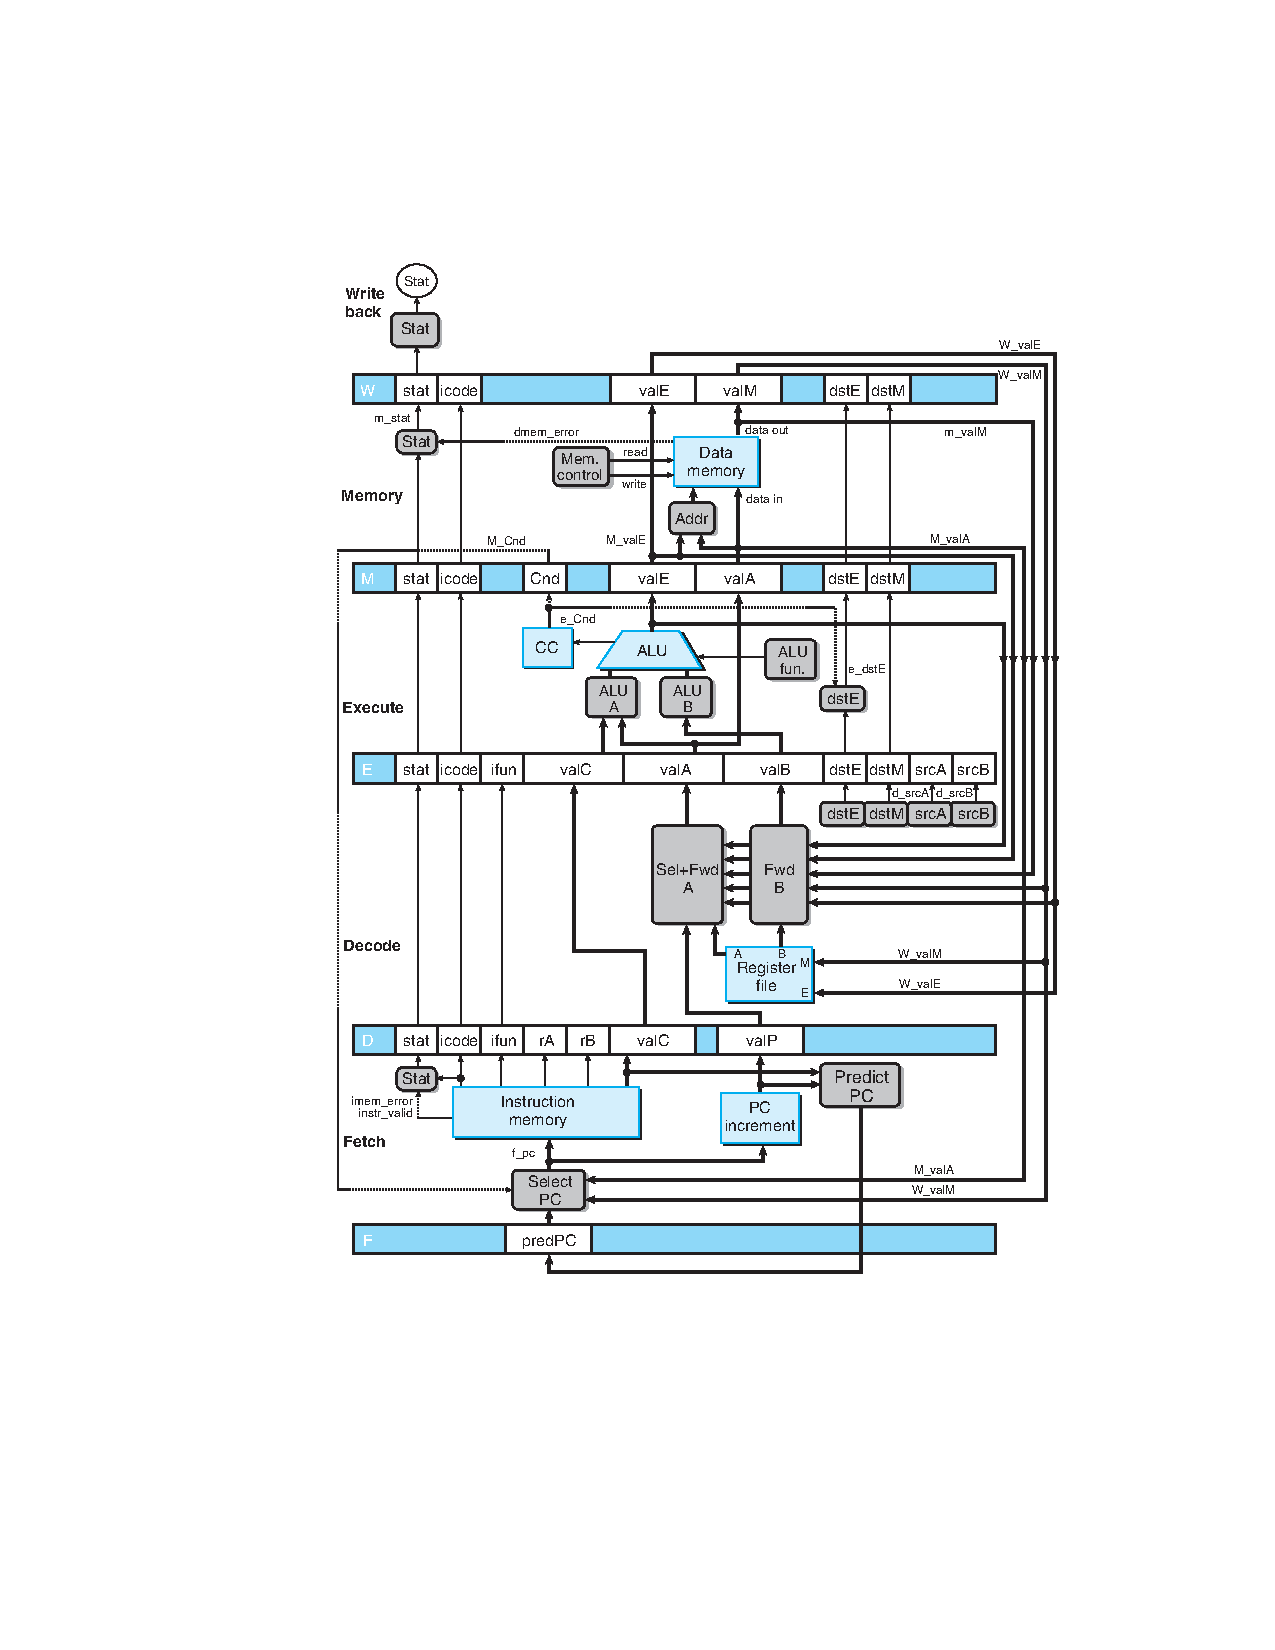
\includegraphics[width=0.75\linewidth]{pipe.pdf}
        \end{figure}
            \qn 该处理器设计采用了前递(forwarding)技术,一定程度上解决了数据相关的问题,在上图中体现在 Sel+FwdA 和 FwdB 部件上。前者输出的信号会存到流水线寄存器 E 的 \verb|valA| 域(即 \verb|E_valA| 信号),请补全该信号的 HCL 语言描述。
            \begin{minted}[frame=single, fontsize=\small]{text}
    int E_valA = [
        D_icode in { ICALL, IJXX } : _________________;
        d_srcA == e_dstE : _________________;
        d_srcA == M_dstM : _________________;
        d_srcA == M_dstE : M_valE;
        d_srcA == W_dstM : W_valM;
        ...
    ];
            \end{minted}
            \qn 如果在该处理器上运行下面的程序,每条指令在不同时钟周期所处的流水线阶段如下表所示。在这种情况下,哪条指令的执行结果会有错误?写出该指令的地址 \rule{2.5cm}{0.25mm}。
            \begin{table}[H]
                \centering
                \begin{tabular}{l|c|c|c|c|c|c|c|c|c|c|c|}
                    \cline{2-12}
                    & 1 & 2 & 3 & 4 & 5 & 6 & 7 & 8 & 9 & 10 & 11 \\ \cline{2-12} 
                    \verb|0x000: irmovl $128, %edx| & F & D & E & M & W &  &  &  &  &  &  \\ \cline{2-12} 
                    \verb|0x006: irmovl $3, %ecx| &  & F & D & E & M & W &  &  &  &  &  \\ \cline{2-12} 
                    \verb|0x00c: rmmovl %ecx, 0(%edx)| &  &  & F & D & E & M & W &  &  &  &  \\ \cline{2-12} 
                    \verb|0x012: irmovl $10, %ebx| &  &  &  & F & D & E & M & W &  &  &  \\ \cline{2-12} 
                    \verb|0x018: mrmovl 0(%edx),%eax| &  &  &  &  & F & D & E & M & W &  &  \\ \cline{2-12} 
                    \verb|0x01e: addl %ebx, %eax| &  &  &  &  &  & F & D & E & M & W &  \\ \cline{2-12} 
                    \verb|0x020: halt| &  &  &  &  &  &  & F & D & E & M & W \\ \cline{2-12} 
                \end{tabular}
            \end{table}
            \qn 如需检测出这个情况,需要增加逻辑电路,用 HCL 语言表达如下:
            \begin{minted}[frame=single, fontsize=\small]{text}
    E_icode in {IMRMOVL, IPOPL} && __________  in { __________ }
            \end{minted}
            \qn 当新增的电路检测出这个情况后,应对各流水线寄存器进行不同的设置,以便在尽可能少影响性能的前提下解决该问题。请填写下表,可选的设置包括 normal/bubble/stall 三种。
            \begin{table}[H]
                \centering
                \begin{tabular}{|c|c|c|c|c|}
                    \hline
                    F & D & E & M & W \\ \hline
                    {\qquad \qquad} & {\qquad \qquad} & {\qquad \qquad} & {\qquad \qquad} & {\qquad \qquad} \\ \hline
                \end{tabular}
            \end{table}
            \qn 如果遇到下面程序代码所展示的情况,该处理器运行时仍然存在问题。因此,还需要新增检测电路。当新增的电路检测出这个情况后,应对各流水线寄存器进行不同的设置,以便在尽可能少影响性能的前提下解决该问题。请填写下表,可选的设置包括 normal/bubble/stall 三种。
            \begin{minted}[frame=single, fontsize=\small]{text}
    0x018: rmmovl   %ecx,0(%edx)
    0x01e: irmovl   $10, %ebx
    0x024: popl     %esp
    0x026: ret
            \end{minted}
            \begin{table}[H]
                \centering
                \begin{tabular}{|c|c|c|c|c|}
                    \hline
                    F & D & E & M & W \\ \hline
                    {\qquad \qquad} & {\qquad \qquad} & {\qquad \qquad} & {\qquad \qquad} & {\qquad \qquad} \\ \hline
                \end{tabular}
            \end{table}
        \proy{2018} Y86 指令 \verb|popl rA| 的 SEQ 实现中,在取指阶段,\verb|valP <- |(\quad),在执行阶段,\verb|valE <- |(\quad)。
        \begin{choices}
            \item \verb|PC+4|、\verb|valA+4|
            \item \verb|PC+4|、\verb|valA+(-4)|
            \item \verb|PC+2|、\verb|valB+4|
            \item \verb|PC+2|、\verb|valB+(-4)|
        \end{choices}
        \proy{2018} 假设已有声明
        \begin{center}
            \tt int i, int sum, int *p, int *q, int *r,const int n = 100, float a[n], float b[n], float c[n], int foo(int), void bar()
        \end{center}
        以下哪项程序优化编译器总是可以进行?
        \vspace{\baselineskip}
        \begin{choices}
            \item \begin{minted}[frame=single, fontsize=\small, linenos]{c}
    // 优化前
    for(i = 0; i < n; ++i) { a[i] += b[i]; a[i] += c[i]; }
    // 优化后
    float tmp;
    for(i = 0; i < n; ++i) { tmp = b[i] + c[i]; a[i] += tmp; }
            \end{minted}
            \item \begin{minted}[frame=single, fontsize=\small, linenos]{c}
    // 优化前
    *p += *q; *p += *r;
    // 优化后
    int tmp;
    tmp = *q + *r;
    *p += tmp;
            \end{minted}
            \item \begin{minted}[frame=single, fontsize=\small, linenos]{c}
    // 优化前
    for(i = 0; i < n; ++i) sum += i * 4;
    // 优化后
    int N = n * 4;
    for(i = 0; i < N; i += 4) sum += i;
            \end{minted}
            \item \begin{minted}[frame=single, fontsize=\small, linenos]{c}
    // 优化前
    for(i = 0; i < foo(n); ++i) bar();
    // 优化后
    int tmp = foo(n);
    for(i = 0; i < tmp; ++i) bar();
            \end{minted}
        \end{choices}
        \proy{2018} 在 PIPE 处理器上运行如下 Y86 代码
        \begin{minted}[frame=single, fontsize=\small]{text}
    .L1
        mrmov   (%eax) %ebx
        addl    %ebx, %ecx
        addl    %ecx, %eax
        xorl    %ecx, %edx
        jne     .L1
        irmov   $1, %eax
        irmov   $1, %eax
        \end{minted}
            \qn 假设上述代码一共循环执行了 $N$ 次后跳出循环,未采用数据前递(data forwarding),分支每次都预测正确,访存每次都命中缓存,命中缓存 时访存需要 1 个周期。请问共需执行多少个周期?
            \qn 假设上述代码一共循环执行了 $N$ 次后跳出循环,采用数据前递(data forwarding),分支每次都预测跳转(taken),访存每次都命中缓存,命中缓存时访存需要 1 个周期。请问共需执行多少个周期?
            \qn 假设上述代码一共循环执行了 $N$ 次后跳出循环($N$ 为偶数),采用数据前递(data forwarding),分支每次都预测不跳转(not taken),数据访存时缓存命中率为 50\%,指令访存全部命中缓存,命中缓存时访存需要 1 个周期,未命中缓存时访存需要 3 个周期。请问共需执行多少个周期?
        \proy{2017} 在 Y86 的 SEQ 实现中,对仅考虑 \verb|IRMMOVQ|、\verb|ICALL|、\verb|IPOPQ|、\verb|IRET| 指令, 对 \verb|mem_addr| 的 HCL 描述正确的是:
        \begin{minted}[frame=single, fontsize=\small]{text}
    word mem_addr = [
        icode in { (1), (2) } : valE;
        icode in { (3), (4) } : valA;
    ];
        \end{minted}
        \begin{choices}
            \item \verb|(1) IRMMOVQ  (2) IPOPQ  (3) IRET     (4) ICALL|
            \item \verb|(1) IRMMOVQ  (2) IRET   (3) IPOPQ    (4) ICALL|
            \item \verb|(1) ICALL    (2) IPOPQ  (3) IRMMOVQ  (4) IRET|
            \item \verb|(1) IRMMOVQ  (2) ICALL  (3) IPOPQ    (4) IRET|
        \end{choices}
        \proy{2017} 关于流水线技术的描述,错误的是: 
        \begin{choices}
            \item 流水线技术能够提高执行指令的吞吐率,但也同时增加单条指令的执行时间。
            \item 增加流水线级数,不一定能获得总体性能的提升。
            \item 指令间数据相关引发的数据冒险,不一定可以通过暂停流水线来解决。
            \item 流水级划分应尽量均衡,吞吐率会受到最慢的流水级影响,均衡的流水线能提高吞吐量。
        \end{choices}
        \proy{2017} 分析 64 位的 Y86 ISA 中新加入的条件内存传送指令:\verb|crmmovqXX| 和 \verb|cmrmovqXX|。\verb|crmmovqXX| 和 \verb|cmrmovqXX| 指令在条件码满足所需要的约束时,分别执行和 \verb|rmmovq| 以及 \verb|mrmovq| 同样的语义。其格式如下:
        \begin{table}[H]
            \tt
            \centering
            \begin{tabular}{c|c|c|c|c|c|}
                \cline{2-6}
                rmmovq & 4 & 0 & rA & rB & D (8 bytes) \\ \cline{2-6} 
                crmmovqXX & 4 & fn & rA & rB & D (8 bytes) \\ \cline{2-6} 
                mrmovq & 5 & 0 & rA & rB & D (8 bytes) \\ \cline{2-6} 
                cmrmovqXX & 5 & fn & rA & rB & D (8 bytes) \\ \cline{2-6} 
            \end{tabular}
        \end{table}
        \qn 请按下表补全每个阶段的操作。需说明的信号可能会包括:\verb|icode|、\verb|ifun|、\verb|rA|、\verb|rB|、\verb|valA|、\verb|valB|、\verb|valC|、\verb|valE|、\verb|valP|、\verb|Cnd|;寄存器堆 \verb|R[]|、存储器 \verb|M[]|、程序计数器 \verb|PC|、条件码 \verb|CC|。其中对存储器的引用必须标明字节数。
        \begin{table}[H]
            \centering
            \begin{tabular}{|c|c|c|}
                \hline
                阶段 & {\qquad} \verb|rmmovq rA, D(rB)| {\qquad} & {\qquad} \verb|cmrmovqXX D(rB), rA| {\qquad} \\ \hline
                取指 & \multicolumn{2}{c|}{\rule{0pt}{10ex}} \\ \hline
                译码 & \multicolumn{2}{c|}{\texttt{valA <- R[rA], valB <- R[rB]}} \\ \hline
                执行 & \rule{0pt}{10ex} & \rule{0pt}{10ex} \\ \hline
                访存 & \rule{0pt}{10ex} & \rule{0pt}{10ex} \\ \hline
                写回 & N/A & \rule{0pt}{10ex} \\ \hline
                更新 \verb|PC| & \multicolumn{2}{c|}{\texttt{PC <- valP}} \\ \hline
            \end{tabular}
        \end{table}
        \qn 为了执行上述新增指令,我们需要改进教材所描述的 PIPE 处理器,在回写(W: Write Back)阶段引入寄存器以保持流水线信号 \rule{2.5cm}{0.25mm} (请参考教材对信号的命名规则书写),以便有条件地更新寄存器内容。在如此改进的 PIPE 处理器上,请写出如下信号的 HCL 代码。
        \begin{minted}[frame=single, fontsize=\small]{text}
    // F_stall 的 HCL 代码:
    (E_icode in {IMRMOVQ, IPOPQ} || (_____1_____))
        && E_dstM in _____2_____ || IRET in _____3_____
    // E_bubble 的 HCL 代码:
    (_____4_____) || (E_icode in {IMRMOVQ, IPOPQ}
        || (_____1_____)) && E_dstM in _____2_____
    // M_bubble 的 HCL 代码:
    m_stat in _____5_____ || W_stat in _____5_____
        \end{minted}
        \qn 对于下面的 Y86 汇编代码,请使用上述条件内存传送指令将其修改为不带跳转的汇编代码序列。假设下面的代码片段在教材所描述的 PIPE 处理器上运行,不考虑该片段前后代码的影响以及高速缓存(cache)失效的情况,假设 \verb|%rsi| 初值为 0, 处理器设计使用总是选择(always taken)的预测策略。原始代码片段预计运行 \rule{2.5cm}{0.25mm} 周期,改进代码片段预计执行 \rule{2.5cm}{0.25mm} 周期。
        \begin{minted}[frame=single, fontsize=\small]{text}
        andq    %rsi %rsi
        jne     L1
        mrmovq  8(%rdx), %rax
        j       L2
    L1:
        mrmovq  8(%rdx), %rbx
    L2:
        addq    %rax, %rbx
        \end{minted}
        \sol 取指部分的填法是很基本的,需要获得 \verb|rA, rB, D|,所以我们写 \verb|icode:ifun <- M1[PC]|、 \verb|rA:rB <- M1[PC+1]|、\verb|valC <- M8[PC+2]| 和 \verb|vavlP <- PC+10|。译码部分也很简单,为 \verb|valA <- R[rA]|、\verb|valB <- R[rB]|。
        
        在执行部分,\verb|rmmovq| 都要计算地址偏移,因此 \verb|valE <- valB+valC|,但是 \verb|cmrmovqXX| 还需要处理条件码,所以还要填 \verb|Cnd <- Cond(CC, ifun)|。最后 \verb|rmmovq| 还需要访存,即 \verb|M8[valE] <- valA|;而 \verb|cmrmovqXX| 除了访存 \verb|valM <- M8[valE]| 之外,还需要条件写回 \verb|if (Cnd) R[rA] <- valM|。
        \proy{2016} 下面对指令系统的描述中,错误的是:
        \begin{choices}
            \item CISC 指令系统中的指令数目较多,有些指令的执行周期很长;而 RISC 指令系统中通常指令数目较少,指令的执行周期都较短。
            \item CISC 指令系统中的指令编码长度不固定;RISC 指令系统中的指令编码长度固定,这样使得 CISC 机器可以获得了更短的代码长度。
            \item CISC指令系统支持多种寻址方式,RISC指令系统支持的寻址方式较少。
            \item CISC 机器中的寄存器数目较少,函数参数必须通过栈来进行传递;RISC 机器中的寄存器数目较多,只需要通过寄存器来传递参数,避免了不必要的存储访问。
        \end{choices}
        \proy{2016} 下面对流水线技术的描述,正确的是:
        \begin{choices}
            \item 流水线技术不仅能够提高执行指令的吞吐率,还能减少单条指令的执行时间。
            \item 不断加深流水线级数,总能获得性能上的提升。
            \item 流水级划分应尽量均衡,吞吐率会受到最慢的流水级影响。
            \item 指令间的数据相关可能会引发流水线停顿,但总是可以通过调度指令来解决。
        \end{choices}
        \proy{2016} 若处理器实现了三级流水线,每一级流水线实际需要的运行时间分别为 \SI{1}{ns}、\SI{2}{ns} 和 \SI{3}{ns},则此处理器不停顿地执行完毕 10 条指令需要的时间为:
        \begin{choices}
            \item \SI{21}{ns}
            \item \SI{12}{ns}
            \item \SI{24}{ns}
            \item \SI{36}{ns}
        \end{choices}
        \sol 首先,每级流水线都是 \SI{3}{ns},然后画出时序图就可以了。一般地,需要时间是一级流水线的总时间,补上一头一尾。这里需要的时间为 $10 \times 3+3+3 = \SI{36}{ns}$。
        \proy{2016} 假设流水线数据通路中的转移预测策略为总是预测跳转。如果转移预测错误,需要恢复流水线,并从正确的目标地址开始取值。其中用来判断转移预测是否正确的信号是 \rule{2.5cm}{0.25mm} 和 \rule{2.5cm}{0.25mm},用来获得正确的目标地址的信号是 \rule{2.5cm}{0.25mm}。
        \begin{choices}
            \item \verb|M_icode   M_Bch   M_valA|
            \item \verb|W_icode   M_Bch   M_valA|
            \item \verb|W_icode   M_Bch   W_valM|
            \item \verb|M_icode   M_Bch   W_valM|
        \end{choices}
        \proy{2016} 请分析 32 位的 Y86 ISA 中新加入的一组条件返回指令 \verb|cretXX|,其格式如下。
        \begin{table}[H]
            \tt
            \centering
            \begin{tabular}{c|c|c|}
                \cline{2-3}
                cretXX & 9 & fun \\ \cline{2-3} 
            \end{tabular}
        \end{table}
        类似 \verb|cmovXX|,该组指令只有当条件码 \verb|Cnd| 满足时,才执行函数返回;如果条件不满足,则顺序执行。
        \qn 若在教材所描述的 SEQ 处理器上执行这条指令,请按下表补全每个阶段的操作。需说明的信号可能会包括:\verb|icode|、\verb|ifun|、\verb|rA|、\verb|rB|、\verb|valA|、\verb|valB|、\verb|valC|、\verb|valE|、\verb|valP|、\verb|Cnd|;寄存器堆 \verb|R[]|、存储器 \verb|M[]|、程序计数器 \verb|PC|、条件码 \verb|CC|。其中对存储器的引用必须标明字节数。如果在某一阶段没有任何操作,请填写 \texttt{none} 指明。
        \begin{table}[H]
            \centering
            \begin{tabular}{|c|c|}
                \hline
                阶段 & {\qquad \qquad \qquad \qquad} \verb|cretXX offset| {\qquad \qquad \qquad \qquad} \\ \hline
                取指 & \rule{0pt}{10ex} \\ \hline
                译码 & \rule{0pt}{10ex} \\ \hline
                执行 & \rule{0pt}{10ex} \\ \hline
                访存 & \rule{0pt}{10ex} \\ \hline
                写回 & \rule{0pt}{10ex} \\ \hline
                更新 \verb|PC| & \rule{0pt}{10ex} \\ \hline
            \end{tabular}
        \end{table}
        \qn 为了执行 \verb|cretXX| 指令,我们需要改进教材所描述的 PIPE 处理器,在 W(Write Back)阶段引入流水线寄存器 \rule{2.5cm}{0.25mm},并将其连接到 PC 选择器(Select PC)以便有条件地更新 PC。假设改进后的处理器总是预测函数返回条件不满足,则如果返回条件满足时,一共会错误取指 \rule{2.5cm}{0.25mm} 条指令。
        \qn 在(2)中改进的 PIPE 处理器上执行 \verb|cretXX| 指令时,发生预测错误时的判断条件为:
        \begin{minted}[frame=single, fontsize=\small]{text}
    (______________ = ICRETXX && ______________) ||
        (______________ = ICRETXX && ______________)
        \end{minted}
        此时各级流水线寄存器的控制信号应如何设置?填写下表。
        \begin{table}[H]
            \centering
            \begin{tabular}{|c|c|c|c|c|}
                \hline
                F & D & E & M & W \\ \hline
                {\qquad \qquad} & {\qquad \qquad} & {\qquad \qquad} & normal & normal \\ \hline
            \end{tabular}
        \end{table}
        \qn 若在 PIPE 处理器上处理器上执行如下代码片段:
        \begin{minted}[frame=single, fontsize=\small]{text}
    0x000: xorl   %eax, %eax
    0x002: popl   %esp
    0x004: cretne
        \end{minted}
            \subqn 是否会发生 load-use 和 misprediction cret 组合的 hazard 情况?
            \subqn 如果此时 \verb|popl %esp| 指令处在流水线的 Execute 阶段,请问此时各级流水线寄存器的控制信号应如何设置?填写下表。
            \begin{table}[H]
                \centering
                \begin{tabular}{|c|c|c|c|c|}
                    \hline
                    F & D & E & M & W \\ \hline
                    {\qquad \qquad} & {\qquad \qquad} & {\qquad \qquad} & normal & normal \\ \hline
                \end{tabular}
            \end{table}
        \sol 本质还是 \verb|ret|,只是需要稍微添加一下条件判断。取指是 \verb|icode:ifun <- M1[PC]|、\verb|valP <- PC+1|。译码需要注意,在 \verb|ret| 中两个值都会被取用,故填写 \verb|valB <- R[%rsp]|、\verb|valA <- R[%rsp]|。
        
        执行阶段是要恢复栈空间,因此为 \verb|valE <- valB+4| 和 \verb|Cnd <- Cond(CC, ifun)|。这里用 \verb|valA| 也可以。访存阶段需要读出返回地址,请注意,这里必须用 \verb|valA|(参看SEQ 实现图中的数据通路),填写 \verb|valM <- M4[valA]|。随后的写回和更新程序计数器的工作主要是关心条件(是否真的要返回了),所以分别是 \verb|if (Cnd) R[%rsp] <- valE| 和 \verb|PC <- Cnd?valM:valP|。
        \proy{2015} 下面有关指令系统设计的描述正确的是:
        \begin{choices}
            \item 采用 CISC 指令比 RISC 指令代码更长。
            \item 采用 CISC 指令比 RISC 指令运行时间更短。
            \item 采用 CISC 指令比 RISC 指令译码电路更加复杂。
            \item 采用 CISC 指令比 RISC 指令的流水线吞吐更高。
        \end{choices}
        \proy{2015} 一个功能模块包含组合逻辑和寄存器,组合逻辑单元的总延迟是 \SI{100}{ps},单个寄存器的延时是 20ps,该功能模块执行一次并保存执行结果,理论上能达到的最短延时和最大吞吐分别是多少?
        \begin{choices}
            \item \SI{20}{ns}、\SI{50}{GIPS}
            \item \SI{120}{ns}、\SI{50}{GIPS}
            \item \SI{120}{ns}、\SI{10}{GIPS}
            \item \SI{20}{ps}、\SI{10}{GIPS}
        \end{choices}
        \proy{2015} 关于流水线技术的描述,错误的是:
        \begin{choices}
            \item 流水线技术能够提高执行指令的吞吐率,但也同时增加单条指令的执行时间。
            \item 减少流水线的级数,能够减少数据冒险发生的几率。
            \item 指令间数据相关引发的数据冒险,都可以通过数据转发来解决。
            \item 现代处理器支持一个时钟内取指、执行多条指令,会增加控制冒险的开销。
        \end{choices}
        \proy{2015} 以下哪些程序优化编译器总是可以自动进行?假设
        \begin{center}
            \tt int i, int j, int A[N], int B[N], float m
        \end{center}
        都是局部变量,\verb|N| 是一个整数型常量,\verb|int foo(int)| 是一个函数。
        \vspace{\baselineskip}
        \begin{choices}
            \item \begin{minted}[frame=single, fontsize=\small, linenos]{c}
    // 优化前
    for (j = 0; j < N; j++) m += i * N * j;
    // 优化后
    int temp = i * N;
    for (j = 0; j < N; j++) m += temp * j;
            \end{minted}
            \item \begin{minted}[frame=single, fontsize=\small, linenos]{c}
    // 优化前
    for (j = 0; j < N; j++) B[i] *= A[j];
    // 优化后
    int temp = B[i];
    for (j = 0; j < N; j++) temp *= A[j];
    B[i] = temp;
            \end{minted}
            \item \begin{minted}[frame=single, fontsize=\small, linenos]{c}
    // 优化前
    for(j = 0; j < N; j++) m = (m + A[j]) + B[j];
    // 优化后
    for(j = 0; j < N; j++) m = m + (A[j] + B[j]);
            \end{minted}
            \item \begin{minted}[frame=single, fontsize=\small, linenos]{c}
    // 优化前
    for(j = 0; j < foo(N); j++) m++;
    // 优化后
    int temp = foo(N);
    for(j = 0; j < temp; j++) m++;
            \end{minted}
        \end{choices}
        \proy{2015} 请分析 Y86 ISA 中新加入的一条指令:\verb|NewJE|,其格式如下。
        \begin{table}[H]
            \centering
            \begin{tabular}{c|c|c|c|c|c|}
                \cline{2-6}
                NewJE & C & 0 & rA & rB & dst \\ \cline{2-6} 
            \end{tabular}
        \end{table}
        其功能为:如果 \verb|R[rA] = R[rB]|,则跳转到 \verb|dst| 继续执行,否则顺序执行。
        \qn 若在教材所描述的 SEQ 处理器上执行这条指令,请按下表补全每个阶段的操作。需说明的信号可能会包括:\verb|icode|、\verb|ifun|、\verb|rA|、\verb|rB|、\verb|valA|、\verb|valB|、\verb|valC|、\verb|valE|、\verb|valP|、\verb|Cnd|;寄存器堆 \verb|R[]|、存储器 \verb|M[]|、程序计数器 \verb|PC|、条件码 \verb|CC|。其中对存储器的引用必须标明字节数。如果在某一阶段没有任何操作,请填写 \texttt{none} 指明。
        \begin{table}[H]
            \centering
            \begin{tabular}{|c|c|}
                \hline
                阶段 & {\qquad \qquad \qquad \qquad} \verb|cretXX offset| {\qquad \qquad \qquad \qquad} \\ \hline
                取指 & \rule{0pt}{10ex} \\ \hline
                译码 & \rule{0pt}{10ex} \\ \hline
                执行 & \rule{0pt}{10ex} \\ \hline
                访存 & \rule{0pt}{10ex} \\ \hline
                写回 & \rule{0pt}{10ex} \\ \hline
                更新 \verb|PC| & \rule{0pt}{10ex} \\ \hline
            \end{tabular}
        \end{table}
        \qn 若在教材所描述的 PIPE 处理器上执行 \verb|NewJE| 指令,如果跳转条件不满足,一共会错误执行 \rule{2.5cm}{0.25mm} 条指令。
        
        为了减小错误预测的代价,现将教材所描述的 PIPE 处理器做如下改进:在 Decode 阶段增加一个比较器,用于判断 \verb|R[rA] = R[rB]| 条件,比较器的输出信号为 \verb|d_equal|。如果相等,则 \verb|d_equal = 1|,反之 \verb|d_equal = 0|。此时,如果执行 \verb|NewJE| 指令时跳转条件不满足,一共会错误执行 \rule{2.5cm}{0.25mm} 条指令。
        \qn 已知在教材所描述的 PIPE 处理器上执行 \verb|jXX| 指令时,发生转移预测错误的判断条件和此时各级流水线寄存器的控制信号如下所示:
        \begin{minted}[frame=single, fontsize=\small]{text}
    E_icode = IJXX & !e_Cnd
        \end{minted}
        \begin{table}[H]
            \centering
            \begin{tabular}{|c|c|c|c|c|}
                \hline
                F & D & E & M & W \\ \hline
                normal & bubble & bubble & normal & normal \\ \hline
            \end{tabular}
        \end{table}
        据此,在第(2)小题所述的改进后的处理器上执行 \verb|NewJE| 指令,发生转移预测错误的判断条件和此时各级流水线寄存器的控制信号应如何设置?
        \begin{minted}[frame=single, fontsize=\small]{text}
    ______________ = INewJE && ______________
        \end{minted}
        \begin{table}[H]
            \centering
            \begin{tabular}{|c|c|c|c|c|}
                \hline
                F & D & E & M & W \\ \hline
                {\qquad \qquad} & {\qquad \qquad} & {\qquad \qquad} & {\qquad \qquad} & {\qquad \qquad} \\ \hline
            \end{tabular}
        \end{table}
        \qn 在第(2)小题所述的改进后的处理器上执行如下代码:
        \begin{minted}[frame=single, fontsize=\small]{text}
    0x000: mrmovl   0(%eax), %edx
    0x006: NewJE    %edx, %eax, t
    0x00c: irmovl   $1, %eax       # Fall through
    0x012: nop
    0x013: nop
    0x014: nop
    0x015: halt
    0x016: t:  irmovl $3, %edx     # Target (Should not execute)
    0x01c: irmovl   $4, %ecx       # Should not execute
    0x022: irmovl   $5, %edx       # Should not execute
        \end{minted}
        会发生 load-use 和 misprediction 组合的 hazard 情况。请问此时,各级流水线寄存器的控制信号应如何设置?
        \begin{table}[H]
            \centering
            \begin{tabular}{|c|c|c|c|c|}
                \hline
                F & D & E & M & W \\ \hline
                {\qquad \qquad} & {\qquad \qquad} & {\qquad \qquad} & normal & normal \\ \hline
            \end{tabular}
        \end{table}
        \qn 在教材 PIPE 处理器设计中,data memory 实际是高速缓存(cache)。假设在执行上述(4)中代码时,\verb|0x000| 指令中的 \verb|0(%eax)| 地址中的数据不在 data memory 中,则 data memory 会将输出信号 \verb|m_datamiss| 置为 1,直到数据从内存中取回到 data memory,再将 \verb|m_datamiss| 置为 0。设 \verb|m_datamiss| 的默认值为 0。这种情况的判断条件如下,请问各级流水线寄存器的控制信号应如何设置?
        \begin{minted}[frame=single, fontsize=\small]{text}
    M_icode in { IMRMOVL, IPOPL } && m_datamiss
        \end{minted}
        \begin{table}[H]
            \centering
            \begin{tabular}{|c|c|c|c|c|}
                \hline
                F & D & E & M & W \\ \hline
                {\qquad \qquad} & {\qquad \qquad} & {\qquad \qquad} & {\qquad \qquad} & {\qquad \qquad} \\ \hline
            \end{tabular}
        \end{table}
        \proy{2014} 若处理器实现了三级流水线,每一级流水线实际需要的运行时间分别为 \SI{2}{ns}、\SI{2}{ns} 和 \SI{1}{ns},则此处理器不停顿地执行完毕 10 条指令需要的时间为:
        \begin{choices}
            \item \SI{21}{ns}
            \item \SI{22}{ns}
            \item \SI{23}{ns}
            \item \SI{24}{ns}
        \end{choices}
        \proy{2014} 关于 RISC 和 CISC 的描述,正确的是:
        \begin{choices}
            \item CISC 指令系统的指令编码可以很短,例如最短的指令可能只有一个字节,因此 CISC 的取指部件设计会比 RISC 更为简单。
            \item CISC 指令系统中的指令数目较多,因此程序代码通常会比较长;而 RISC 指令系统中通常指令数目较少,因此程序代码通常会比较短。
            \item CISC 指令系统支持的寻址方式较多,RISC 指令系统支持的寻址方式较少,因此用 CISC 在程序中实现访存的功能更容易。
            \item CISC 机器中的寄存器数目较少,函数参数必须通过栈来进行传递;RISC 机器中的寄存器数目较多,只需要通过寄存器来传递参数。
        \end{choices}
        \proy{2014} 关于流水线技术的描述,正确的是:
        \begin{choices}
            \item 指令间数据相关引发的数据冒险,一定可以通过暂停流水线来解决。
            \item 流水线技术不仅能够提高执行指令的吞吐率,还能减少单条指令的执行时间。
            \item 增加流水线的级数,一定能获得性能上的提升。
            \item 流水级划分应尽量均衡,不均衡的流水线会增加控制冒险。
        \end{choices}
        \proy{2014} 下面关于程序性能的说法中,哪个是正确的?
        \begin{choices}
            \item 处理器内只要有多个功能部件空闲,就能实现指令并行,从而提高程序性能。
            \item 同一个任务采用时间复杂度为 $O(\log N)$ 算法一定比采用复杂度为 $O(N)$ 算法的执行时间短。
            \item 转移预测总是能带来好处,不会产生额外代价,对提高程序性能有帮助。
            \item 增大循环展开(loop unrolling)的级数,有可能降低程序的性能(即增加执行时间)。
        \end{choices}
        \proy{2014} 请分析 Y86 ISA 中新加入的一条指令:\verb|caddXX| 条件加法。其功能可以参考 \verb|add| 和 \verb|cmovXX| 两条指令。
        \begin{table}[H]
            \centering
            \begin{tabular}{c|c|c|c|c|}
                \cline{2-5}
                caddXX & C & fn & rA & rB \\ \cline{2-5} 
            \end{tabular}
        \end{table}

        若在教材所描述的 SEQ 处理器上执行这条指令,请按下表补全每个阶段的操作。需说明的信号可能会包括:\verb|icode|、\verb|ifun|、\verb|rA|、\verb|rB|、\verb|valA|、\verb|valB|、\verb|valC|、\verb|valE|、\verb|valP|、\verb|Cnd|;寄存器堆 \verb|R[]|、存储器 \verb|M[]|、程序计数器 \verb|PC|、条件码 \verb|CC|。其中对存储器的引用必须标明字节数。如果在某一阶段没有任何操作,请填写 \texttt{none} 指明。
        \begin{table}[H]
            \centering
            \begin{tabular}{|c|c|}
                \hline
                阶段 & {\qquad \qquad \qquad \qquad} \verb|caddXX offset| {\qquad \qquad \qquad \qquad} \\ \hline
                取指 & \rule{0pt}{10ex} \\ \hline
                译码 & \rule{0pt}{10ex} \\ \hline
                执行 & \rule{0pt}{10ex} \\ \hline
                访存 & \rule{0pt}{10ex} \\ \hline
                写回 & \rule{0pt}{10ex} \\ \hline
                更新 \verb|PC| & \rule{0pt}{10ex} \\ \hline
            \end{tabular}
        \end{table}
    \end{problems}